\documentclass{article}\usepackage[]{graphicx}\usepackage[]{color}
%% maxwidth is the original width if it is less than linewidth
%% otherwise use linewidth (to make sure the graphics do not exceed the margin)
\makeatletter
\def\maxwidth{ %
  \ifdim\Gin@nat@width>\linewidth
    \linewidth
  \else
    \Gin@nat@width
  \fi
}
\makeatother

\definecolor{fgcolor}{rgb}{0.345, 0.345, 0.345}
\newcommand{\hlnum}[1]{\textcolor[rgb]{0.686,0.059,0.569}{#1}}%
\newcommand{\hlstr}[1]{\textcolor[rgb]{0.192,0.494,0.8}{#1}}%
\newcommand{\hlcom}[1]{\textcolor[rgb]{0.678,0.584,0.686}{\textit{#1}}}%
\newcommand{\hlopt}[1]{\textcolor[rgb]{0,0,0}{#1}}%
\newcommand{\hlstd}[1]{\textcolor[rgb]{0.345,0.345,0.345}{#1}}%
\newcommand{\hlkwa}[1]{\textcolor[rgb]{0.161,0.373,0.58}{\textbf{#1}}}%
\newcommand{\hlkwb}[1]{\textcolor[rgb]{0.69,0.353,0.396}{#1}}%
\newcommand{\hlkwc}[1]{\textcolor[rgb]{0.333,0.667,0.333}{#1}}%
\newcommand{\hlkwd}[1]{\textcolor[rgb]{0.737,0.353,0.396}{\textbf{#1}}}%

\usepackage{framed}
\makeatletter
\newenvironment{kframe}{%
 \def\at@end@of@kframe{}%
 \ifinner\ifhmode%
  \def\at@end@of@kframe{\end{minipage}}%
  \begin{minipage}{\columnwidth}%
 \fi\fi%
 \def\FrameCommand##1{\hskip\@totalleftmargin \hskip-\fboxsep
 \colorbox{shadecolor}{##1}\hskip-\fboxsep
     % There is no \\@totalrightmargin, so:
     \hskip-\linewidth \hskip-\@totalleftmargin \hskip\columnwidth}%
 \MakeFramed {\advance\hsize-\width
   \@totalleftmargin\z@ \linewidth\hsize
   \@setminipage}}%
 {\par\unskip\endMakeFramed%
 \at@end@of@kframe}
\makeatother

\definecolor{shadecolor}{rgb}{.97, .97, .97}
\definecolor{messagecolor}{rgb}{0, 0, 0}
\definecolor{warningcolor}{rgb}{1, 0, 1}
\definecolor{errorcolor}{rgb}{1, 0, 0}
\newenvironment{knitrout}{}{} % an empty environment to be redefined in TeX

\usepackage{alltt}
%\usepackage{animate}
\usepackage[round]{natbib}
\usepackage[nolists]{endfloat}
\usepackage[width = 5in]{geometry}
\usepackage{caption, amsmath, graphicx, setspace, multirow, color, hyperref, array}
\title{Mixed GWR Simulation Write-up}
\author{Aaron Swoboda}
\IfFileExists{upquote.sty}{\usepackage{upquote}}{}
\begin{document}
\maketitle

What are our research questions? Basically:
\begin{enumerate}
\item Can we find the ``true'' model among the eight different possibilities with three model parameters?
\item Are there differences in the results based on the metric used?
\item What happens as we change the sample size and amount of error in the model?
\item How much does it really matter if we are concerned with coefficient estimates?
  \begin{itemize}
  \item How well does our selected model perform as measured by beta RMSE?
  \item Does our model perform better when we select the correct model?
  \item Can we control for whether we selected a model with the correct spatial variation for a given parameter?
  \end{itemize}
\item What about using bandwidth size as a dependent variable?
\item What happens when we use other decision tools to help with model selection? (Monte Carlo simulations and test statistics)
\end{enumerate}




\section{Background}

Imagine a simple linear model,
\begin{equation}\label{eq:simpleOLS}
Y = \beta _0 + \beta _1 *X_1 + \beta _2 * X_2 + \epsilon .
\end{equation}
In addition to the three variables listed above ($Y$, $X_1$, and $X_2$), assume we know the geographical location for each of our $N$ observations. Thus, our data consists of an $N x 5$ matrix, where $Y$ may be house prices, $X_1$ and $X_2$ could be the living space and lot size associated with each house, and the final two columns determine the location of the observations (for instance, latitude and longitude, or distances north and east from a prescribed point).

The simple model in \eqref{eq:simpleOLS} exemplifies spatial stationarity in the parameters: the $\beta$ coefficients are constant over space. Alternatively, the coefficients could exhibit spatial non-stationarity, in which case one, two, or all three of the $\beta$ coefficients are a function of location. This has a natural interpretation in the current real estate example: location matters. However, location can matter in different ways. For instance, if the value of land varies over space, then we would expect the coefficient on lot size to vary over space, while it is also possible that the intercept varies over space to reflect variation in prices of similar houses in different locations. 

While it is possible to parameterize the variation in coefficients, for instance researchers often (CITATION?) include a variable measuring the distance from an observation to an important amenity such as the Central Business District and then this distance variable could be interacted with variables whose value are predicted to vary over space. However, it is not implausible to believe that the variation in coefficients might not be easily parameterized (for instance, if land values are a non-monotonic function of distance). Researchers may instead interact variables with fixed effects for cities or census tracts. However, such strategies require the analyst to make assumptions that severely limit the type and degree of variation in the parameters. For instance, interaction terms with geographic boundaries assume discrete differences in the value of parameters across the boundaries, while instead the parameters may instead be a continuous function of location.

\subsection{Local Regression to the Rescue?}
Locally Weighted Regression (also known as Geographically Weighted Regression) is one possible solution to the challenge presented by spatially non-stationary regression coeffiecients. Locally Weighted Regression (LWR) techniques (also known as Geographically Weighted Regression) are described in detail by \citet{Cleveland1988}, \citet{Brunsdon1998b}, \citet{Fotheringham2002}, and others. It is a weighted least squares methodology in which regression coefficients are estimated over space as a function of the local data as described in Equation~\eqref{eq:LWRbeta},
\begin{equation}\label{eq:LWRbeta}
\hat{\beta}_i = (X'W_iX)^{-1}X'W_iY,
\end{equation}
where X is a $N \times 2$ matrix of independent variables, $W_i$ is the $N \times N$ weights matrix, and Y is the $N \times 1$ vector of dependent variable values. The weights matrix, $W_i$ is a diagonal matrix where element $w_{jj}$ denotes the weight that the $j^{th}$ data point will receive in the regression coefficients estimated at location $i$ in the dataset. We employ a bi-square weights function and a k-nearest neighbor bandwidth approach as described in equation~\eqref{eq:weights}, 
\begin{equation}\label{eq:weights}
w_{jj}=\left[1-\left(\frac{d_{ij}}{d_{k}}\right)^2 \right]^2 \textrm{ if  }d_{ij}<d_{ik}\textrm{, otherwise = 0},
\end{equation}
where $d_{ij}$ denotes the distance between observations $i$ and $j$, and $d_{ik}$ is the distance from observation $i$ to the $k^{th}$ nearest observation. This function assigns weights close to 1 for data points near observation $i$, weights positive but closer to zero for observations farther away, and zero for all $n-k$ observations farther away than the $k^{th}$ nearest observation. 

A key decision in estimating LWR models is choosing the number of observations to include in the bandwidth. Bandwidths that are too large in the presence of spatial non-stationarity create bias in the regression estimates (the large bandwidth creates weights matrices that are similar over space and therefore the regression coefficients are forced to be similar when they should vary over space). Bandwidths that are too small add unneccessary error in our estimates by excluding informative observations. Often, researchers choose a bandwidth my minimizing a cross validation metric. This choice is further complicated in the context of mixed models where only some coefficents exhibit spatial stationarity (in contrast to standard models in which all coefficients are treated as spatially stationary or LWR models in which no coefficients are treated as stationary). Little is known about model performance when models are selected across multiple mixed models and among multiple different potenial bandwidth sizes.

\section{Title Needed}

This paper uses simulated data generated under multiple conditions to begin to answer some of the outstanding questions in the area of geographically mixed models. We compare four important cross-validation/information criteria: Leave One Out Cross Validation (LOOCV), Generalized Cross Validation (GCV), Standardized Cross Validation (SCV), and the Akaike Information Criterion (AIC). How frequently can researchers utilizing these metrics identify the correct model among the various possible combinations? Are certain metrics more/less prone to false positive/negatives? Do they suggest no spatial variation when in fact it exists? Do they suggest spatial variation when in fact there is not? 

Perhaps the most common cross validation metric used in the literature (how many citations?) is the Leave One Out Cross Validation score (LOOCV), which is calculated as follows,
\begin{equation}\label{eq:LOOCV}
LOOCV = \frac{1}{N} \sqrt{\sum _{i = 1}^{N} (y - \hat{y}_{\neq i})^2},  
\end{equation}
where $\hat{y}_{\neq i}$ represents the dependent variable estimate for observation $i$ while excluding observation $i$ from the regression. This prevents the observation from having undue influence in the regression with small bandwidths and overfitting the model. Such a model, while intuitively appealing, can be computationally expensive, as regressions must be estimated first while excluding individual observations to calculate the LOOCV and then again while including the observation to obtain the regression coefficients.

An alternative cross validation metric is known as the Generalized Cross Validation (GCV) score, which only requires calculating the regressions once per location and explicitly calculates the leverage each observation has over the regression coefficients. The GCV score calculation is detailed in equation~\eqref{eq:GCV},
\begin{equation}\label{eq:GCV}
n*\sum_{i=1}^{n}\frac{(y_i-\hat{y}_i)^2}{(n-v_1)^2}, 
\end{equation} 
where $\hat{y}_i$ is the predicted dependent variable value for observation $i$, and $v_1$ can be interpreted as the ``effective number of model parameters,'' and calculated as $v_1=$tr(\textbf{S}), where the matrix \textbf{S} is the ``hat matrix'' which maps $y$ onto $\hat{y}$,
                   \begin{equation}
                   \hat{y}=\textbf{S}y,
                   \end{equation}
                   and each row of \textbf{S}, $r_i$ is given by:
                  \begin{equation}
                   r_i=X_i(X'W_iX)^{-1}X'W_i.
                   \end{equation}
The GCV score is a convenient model selection metric that rewards models that provide a good fit to the data, while penalizing models with a greater number of model parameters \citep{Loader1999, McMillen2010}.  \citep{Paez2011, McMillen2010, McMillen2012}. 

The Standardized Cross Validation Score was suggested by (CITATION)

AIC

\subsection{Experimental Design}

We generate data in the following format:
\begin{equation}
Y = \beta _0(location) + \beta _1(location) *X_1 + \beta _2(location) * X_2 + \epsilon ,
\end{equation}
where sometimes the coefficient is in fact stationary, $\beta _m(location) = \beta$, and other times it is non-stationary, $\beta _m (location_p) \neq \beta _m (location_q)$. With three coefficients, $m = \{0, 1, 2\}$, each having the possibility of being stationary or not, there are eight different possible combinations, ranging from (stationary, stationary, stationary) to (non-stationary, non-stationary, non-stationary).

We generate data using all eight different combinations and then estimate all eight possible LWR models across seven different bandwidth sizes. We then calculate different Cross-Validation metrics and compare their values across models and bandwidths. 

We have three different values for each coefficient in our DGP, no variation, some variation, and more variation.

We also change the sample size of our data as well as the variance of the model error term.

\section{Simulation Results}

We begin by showing the results for the data generation process with no spatial variation for any of the coeffients. To denote that $\beta _0$, $\beta _1$, and $\beta _2$ are each ``Global'' (rather than ``Local'') we label this model ``GGG''. At this point, we are most interested in which model, among the eight possible, would be chosen by minimizing the various metrics, AIC, GCV, SCV, and LOOCV. The following table shows the different selection metrics in columns and the eight different models (GGG, LGG, GLG, GGL, LLG, LGL, GLL, and LLL) in the rows. The values in each cell represent the percentage of the experiments that the metric in the column was minimized by the row model. Each column sums to 100 (subject to rounding error). 

For instance, the table shows that 72 percent of the time when the true model contained no spatial variation, the LOOCV metric was minimized by the `GGG' model, while the majority of the remaining 28 percent of the time the LOOCV was minimized by the `LGG', `GLG', and `GGL' models. In other words, almost three-fourths of the time the LOOCV was minimized using the model that was ``correct'' across all three coefficients and only 5 percent of the time was this metric minimized by a model ``wrong'' about two or three of the coefficients at the same time.

On the other hand, the table shows that the AIC and GCV metrics were almost never minimized by the true model ($<0.5$ percent). Instead, the models ``chosen'' by these metrics were approximately evenly split among `LGG', `GLG', and `GGL', each of which is wrong about one of the coefficients (a coefficient is believed to be local when it is global). The SCV metric chooses the true model more than the AIC or GCV metrics (8 percent vs. $<0.5$ percent), but far less than the LOOCV metric. However, it also is `wrong' about two or more coefficients in almost 20 percent of these cases (compared to 1 [AIC], 3 [GCV], and 4 [LOOCV]).

The final three columns show which model minimized the Root Mean Square Error for each of the three coefficients in our model. These metrics are only available because of the nature of the experiment - we know the true values of the coefficients in the underlying true model and so can compare the estimated coefficients to their true values. The results are startling. The true model, `GGG' yields that most accurate estimates of the coefficient in question less than 10 percent of the time. Further inspection shows an interesting pattern. For each of our three coefficients, the model with the most accurate estimates is the model that is correct about the global nature of the coefficient in question, but uses a local model for the other two coefficients. For instance, the most accurate estimates of $\beta _0$ occur almost one-third of the time when using the `GLL' model. In other words, the model that is most likely to have the most accurate estimates for a given coefficient is consistently NOT the correct model, although it tends to correctly identify the spatial (non-)stationarity of the coefficient in question.


As a reminder, four of these are available to a researcher with actual data, while the $\textrm{RMSE}_{\hat{\beta _0}}$ etc are only available to 


We have seven different ways to pick the ``best'' model (the AIC, GCV, SCV, LOOCV, and RMSEs for the three different coefficients). Here are tables showing the relative frequency (in percentage) that each model number was selected by optimizing a given metric. Note that the columns in the following tables may not sum exactly to 100 due to rounding.




\begin{knitrout}
\definecolor{shadecolor}{rgb}{0.969, 0.969, 0.969}\color{fgcolor}\begin{kframe}
\begin{verbatim}
##         Metric
## ModelNum AIC GCV SCV LOOCV B0RMSE B1RMSE B2RMSE
##        1   0   0   8    72      6      6      7
##        2  28  28  29     7      3     23     24
##        3  37  36  22     8     22      4     24
##        4   0   1   5     1      5      3     33
##        5  34  33  22     8     23     23      3
##        6   1   1   5     2      5     36      2
##        7   0   1   8     1     32      4      4
##        8   0   0   1     0      4      2      3
\end{verbatim}
\end{kframe}
\end{knitrout}

Let's visualize these results.



\begin{figure}
  \makebox[\textwidth][c]{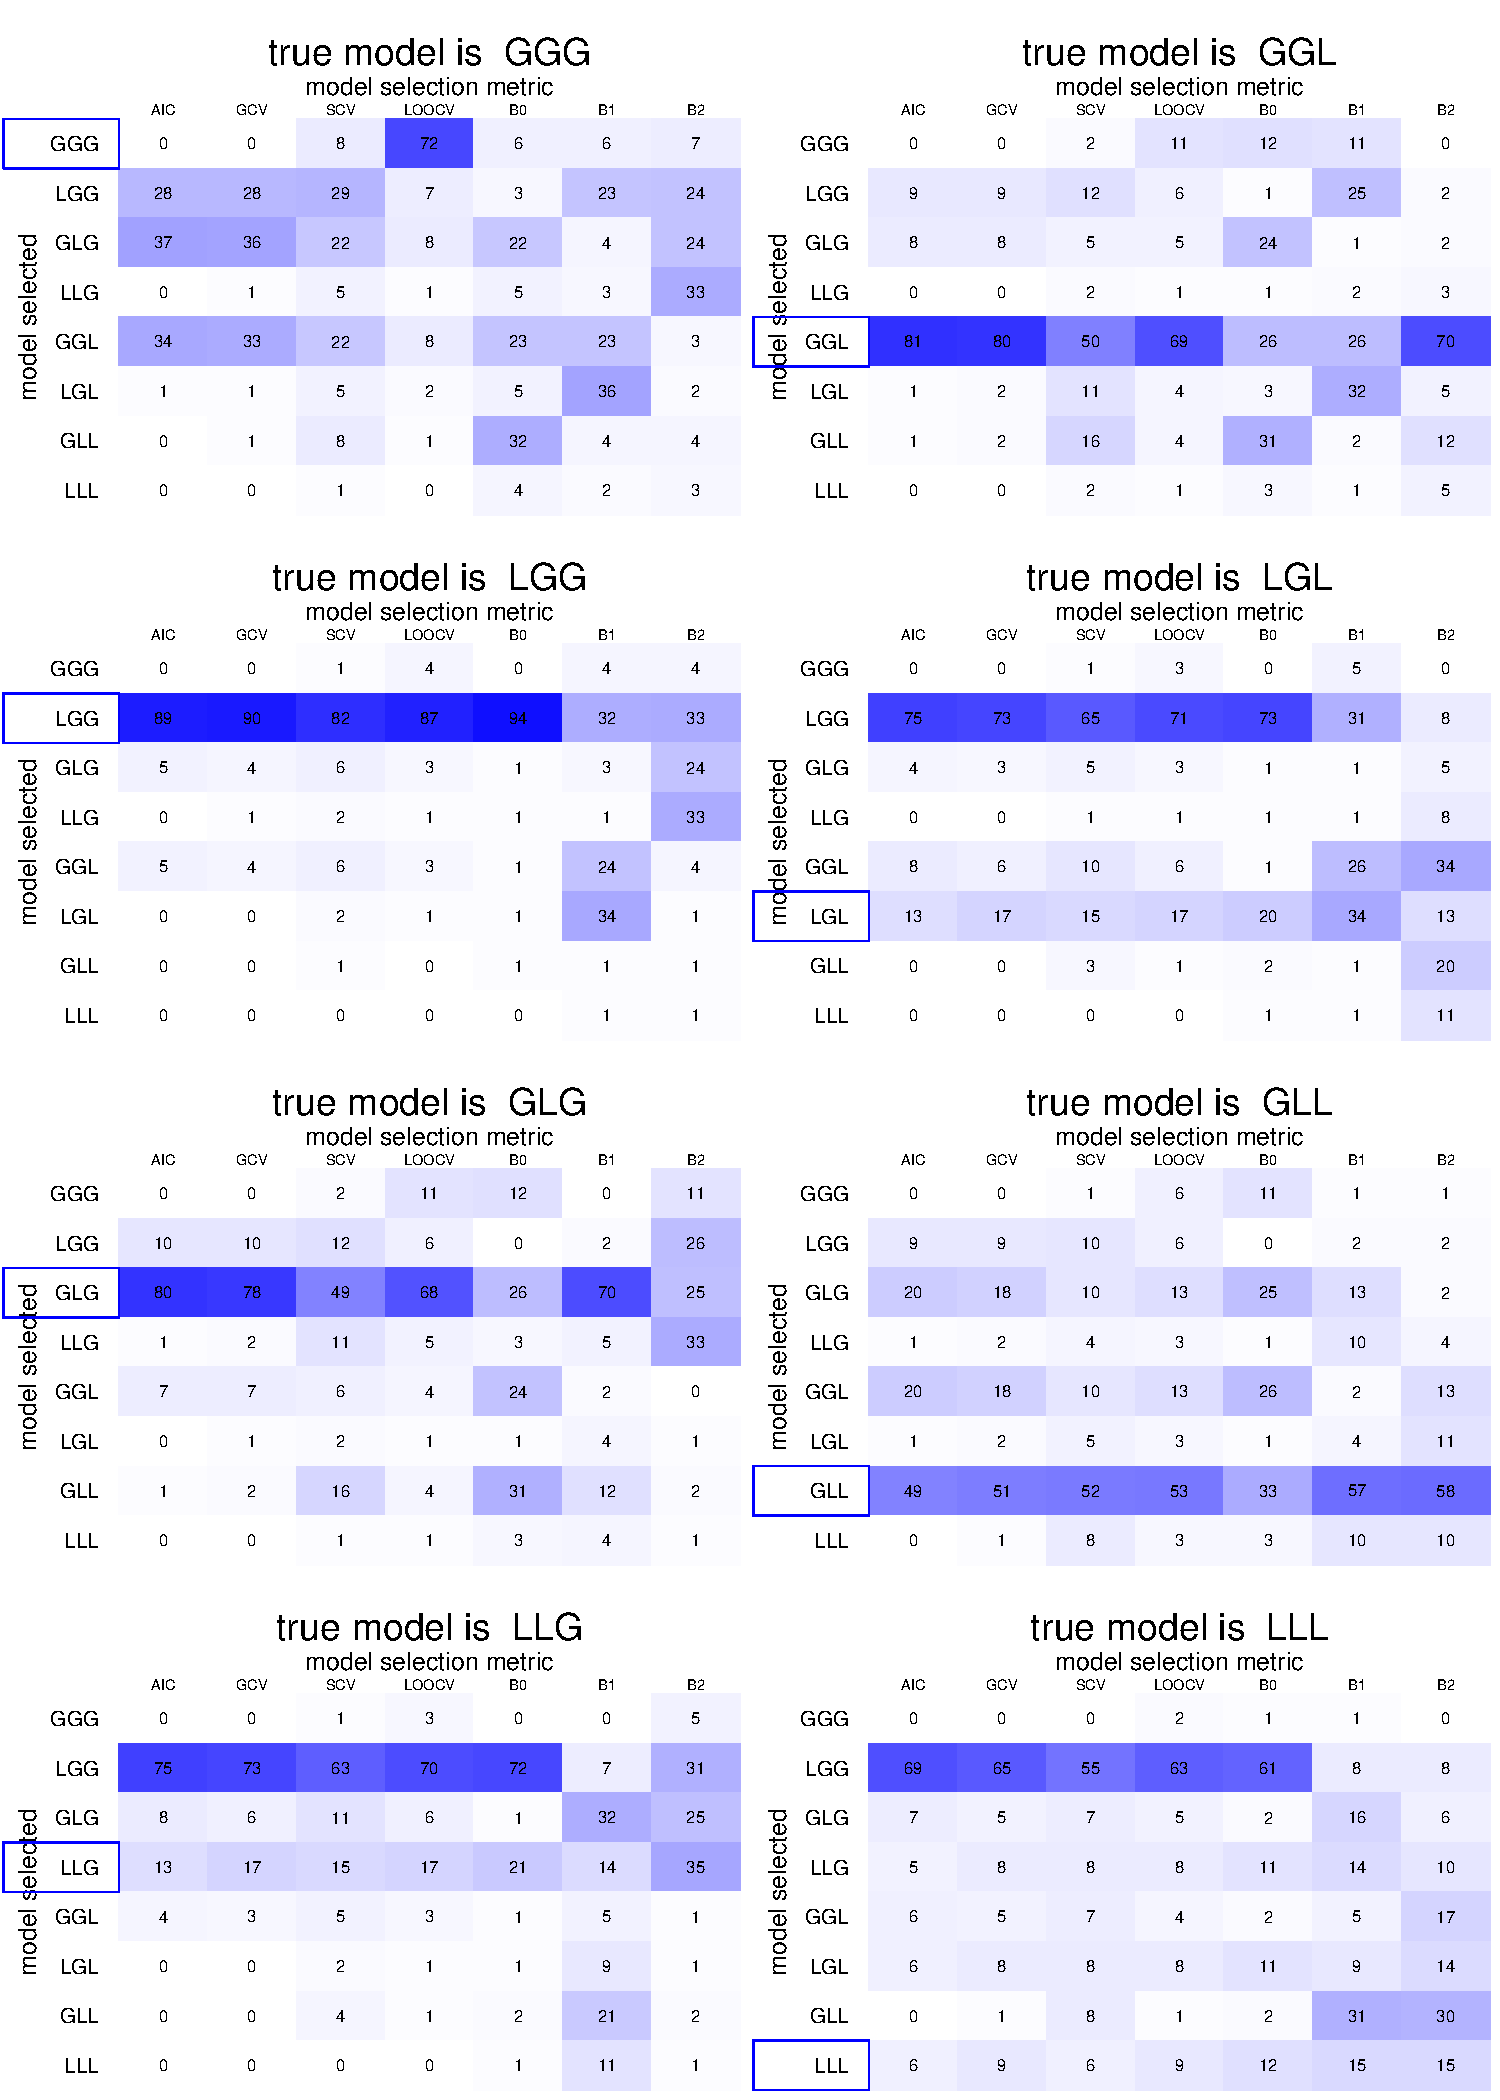
\includegraphics[width = 1.2\textwidth]{figure/ModelSelectionFigures.pdf}}
\caption{This figure shows }
\label{fig:}
\end{figure}

Another visualization idea: put the eight tables in a 4 x 3 matrix with the rows denoting how many coefficients in the true DGP are ``local''. Top row contains the `GGG' model, middle `LGG' `GLG' and 'GGL'... bottom row contains the `LLL' model. Will have to use `layout' function in R to leave the blank spots

The results of the previous tables must be taken with a grain of salt, as there could times when a ``true'' model may include variation in a coefficient, but the degree of non-stationarity in the coefficient may be small. In such cases, choosing an incorrect model (such as one that keeps such a coefficient constant) may not be such a big problem. Alternatively, the ``best'' model may have some local coefficients, but the bandwidth chosen might be large and therefore implying the model allows for very little variation in the coefficients.

Some patterns clearly emerge. 
\begin{itemize}
\item The AIC and GCV metrics \emph{never} select Model 1, even when it is the actual model.
\item There are several occasions where the model/bandwidth combination with the smallest RMSE is not the ``correct'' model.
\end{itemize}

% \subsection{Coefficient Formulation}
% 
% Even if an incorrect model is chosen, the model may yield accurate estimates of the coefficients. In each run of the simulation we estimated 50 different model/bandwidth combinations (seven different bandwidths for each of the seven models with at least one coefficient varying over space, plus the standard OLS model). We calculate the Root Mean Squared Error for each model and can rank these values. For instance, it is possible, and often the case, that the ``wrong'' model yields the most accurate estimates of a coefficient among all of the models implemented.
% 
% 
% <<BetaRankTabulations, fig.width=4, fig.height=6, fig.show='animate', aniopts='autoplay,loop,controls', interval=2>>=
% colMat = matrix("black", 8, 3)
% colMat[as.matrix(models)=="yes"] = "red"
% par(oma = c(0, 2, 3, 0))
% par(mar = rep(1, 4))
% for (i in 1:8) {
%   #i = 1
%   layout(matrix(1:12, 4, 3, byrow=T))
%   temp2 = which(mcOutput[1, "True Model", ] == i)
%   inputMetrics = c("AIC", "GCV", "SCV", "LOOCV")
%   inputStats = c("B0RMSE Rank", "B1RMSE Rank", "B2RMSE Rank")
%   for (j in 1:4) {
%     for (k in 1:3) {
%       temp3 = mcOutput[inputMetrics[j], inputStats[k], temp2]
%       #summary(temp3)
%       hist(temp3, xlim = c(0, 50), breaks = 5*(0:10), 
%            col = ifelse(colMat[i, k]=="red", "red", "grey85"),
%        axes = F, ylab = "rel freq", xlab = "rank", main = "")
%     }
%   }
%   mtext(text=paste0("Model #", i, "(non-stationary parameters in red"), 
%         side=3, outer=TRUE, line = 1.8)
%   mtext(inputMetrics, at = seq(.875, .125, length.out=4), side = 2, outer = T)
%   mtext(paste0("B", 0:2), at = seq(.17,.83, length.out=3), 
%         side = 3, outer = T, line = 0, col = colMat[i, ])
% }
% 
% @
% 
% 
% \section{Accuracy of Beta Estimates}
% 
% During the experiment we calculated the Root Mean Squared Error the estimated coefficients for all models. We then ranked each model from smallest to largest RMSEs and collected the RMSE values and ranks for all models that minimized one of the model selection criteria and the model with the smallest RMSE for this coefficient. 
% 
% Let's see if there is a relationship between the RMSE values/ranks and the parameters we modified in the experiment.
% 
% <<makeData>>=
% #   temp2 = which(mcOutput[1, "True Model", ] == i)
% #   inputMetrics = c("AIC", "GCV", "SCV", "LOOCV")
% #   inputStats = c("B0RMSE Rank", "B1RMSE Rank", "B2RMSE Rank")
% # temp3 = mcOutput[inputMetrics[j], inputStats[k], temp2]
% myVars = c("B0RMSE",     "B1RMSE",     "B2RMSE",
%            "B0RMSE Rank",  "B1RMSE Rank",  "B2RMSE Rank", 
%            "Sample Size",  "Error", "True Model",
%            "B0 SpVar", "B1 SpVar", "B2 SpVar", "Model Number")
% rankData1 = as.data.frame(t(mcOutput["AIC", myVars, ]))
% rankData1$Metric = "AIC"
% 
% rankData2 = as.data.frame(t(mcOutput["GCV", myVars, ]))
% rankData2$Metric = "GCV"
% 
% rankData3 = as.data.frame(t(mcOutput["SCV", myVars, ]))
% rankData3$Metric = "SCV"
% 
% rankData4 = as.data.frame(t(mcOutput["LOOCV", myVars, ]))
% rankData4$Metric = "LOOCV"
% 
% rankData = rbind(rankData1, rankData2, rankData3, rankData4)
% 
% rankData$samplesize = rankData[, "Sample Size"]
% rankData$error = as.factor(rankData$Error)
% rankData$truemodel = as.factor(rankData[, "True Model"])
% rankData$B0sv = as.factor(rankData[, "B0 SpVar"])
% rankData$B1sv = as.factor(rankData[, "B1 SpVar"])
% rankData$B2sv = as.factor(rankData[, "B2 SpVar"])
% rankData$metric = as.factor(rankData$Metric)
% names(rankData)[which(names(rankData)=="Model Number")] = "selectedmodel"
% 
% @
% 
% \subsection{RMSE Values}
% 
% <<RMSEregression011>>=
% RMSEregression0 <- lm(B0RMSE ~ samplesize + metric + B0sv + B1sv + B2sv + error, 
%                data = rankData)
% summary(RMSEregression0)
% @
% <<RMSEregression111>>=
% RMSEregression1 <- lm(B1RMSE ~ samplesize + metric + B0sv + B1sv + B2sv + error, 
%                data = rankData)
% summary(RMSEregression1)
% @
% <<RMSEregression211>>=
% RMSEregression2 <- lm(B2RMSE ~ samplesize + metric + B0sv + B1sv + B2sv + error, 
%                data = rankData)
% summary(RMSEregression2)
% @
% 
% Now I'd like to add a variable along the lines of ``does the selected model correctly identify whether the variable is non-stationary?''
% 
% <<identifySV>>=
% TrueModelBeta0sv = c(2, 4, 6, 8)
% TrueModelBeta1sv = c(3, 4, 7, 8)
% TrueModelBeta2sv = 5:8
% 
% ModelBetaSV.selected.true = function(TrueModelBetasv) {
%   temp = rankData$truemodel %in% TrueModelBetasv
%   temp2 = rankData$selectedmodel %in% TrueModelBetasv
%   ModelBetaSVCorrect <- temp == temp2
%   ModelBetaSVCorrect
% }
% 
% rankData$ModelBeta0svTrue = ModelBetaSV.selected.true(TrueModelBeta0sv)
% rankData$ModelBeta1svTrue = ModelBetaSV.selected.true(TrueModelBeta1sv)
% rankData$ModelBeta2svTrue = ModelBetaSV.selected.true(TrueModelBeta2sv)
% @
% 
% <<RMSEregression012>>=
% RMSEregression0 <- lm(B0RMSE ~ samplesize + metric + B0sv + B1sv + B2sv + error + ModelBeta0svTrue, 
%                data = rankData)
% summary(RMSEregression0)
% @
% <<RMSEregression112>>=
% RMSEregression1 <- lm(B1RMSE ~ samplesize + metric + B0sv + B1sv + B2sv + error + ModelBeta1svTrue, 
%                data = rankData)
% summary(RMSEregression1)
% @
% <<RMSEregression212>>=
% RMSEregression2 <- lm(B2RMSE ~ samplesize + metric + B0sv + B1sv + B2sv + error + ModelBeta2svTrue, 
%                data = rankData)
% summary(RMSEregression2)
% @
% 
% Now add all three:
% 
% <<RMSEregression013>>=
% RMSEregression0 <- lm(B0RMSE ~ samplesize + metric + B0sv + B1sv + B2sv + error + ModelBeta0svTrue, 
%                data = rankData)
% summary(RMSEregression0)
% @
% <<RMSEregression113>>=
% RMSEregression1 <- lm(B1RMSE ~ samplesize + metric + B0sv + B1sv + B2sv + error + ModelBeta1svTrue, 
%                data = rankData)
% summary(RMSEregression1)
% @
% <<RMSEregression213>>=
% RMSEregression2 <- lm(B2RMSE ~ samplesize + metric + B0sv + B1sv + B2sv + error + ModelBeta2svTrue, 
%                data = rankData)
% summary(RMSEregression2)
% @
% 
% \subsection{RMSE Rank}
% How are the various parameters related to the results of the $\beta _0$ ranking?
% <<regression021>>=
% rankData$B0rank = rankData[, "B0RMSE Rank"]
% rankData$B1rank = rankData[, "B1RMSE Rank"]
% rankData$B2rank = rankData[, "B2RMSE Rank"]
% rankLM <- lm(B0rank ~ samplesize + metric + B0sv + B1sv + B2sv + error, 
% data = rankData)
% summary(rankLM)
% @
% 
% How are the various parameters related to the results of the $\beta _1$ ranking?
% <<regression121>>=
% rankLM <- lm(B1rank ~ samplesize + metric + B0sv + B1sv + B2sv + error, data = rankData)
% summary(rankLM)
% @
% 
% How are the various parameters related to the results of the $\beta _2$ ranking?
% <<regression221>>=
% rankLM <- lm(B2rank ~ samplesize + metric + B0sv + B1sv + B2sv + error, data = rankData)
% summary(rankLM)
% @
% 
% 
% Now add in whether or not the correct model was specified.
% <<regression022>>=
% rankLM <- lm(B0rank ~ samplesize + metric + B0sv + B1sv + B2sv + error + ModelBeta0svTrue, data = rankData)
% summary(rankLM)
% @
% 
% How are the various parameters related to the results of the $\beta _1$ ranking?
% <<regression122>>=
% rankLM <- lm(B1rank ~ samplesize + metric + B0sv + B1sv + B2sv + error + ModelBeta1svTrue, data = rankData)
% summary(rankLM)
% @
% 
% How are the various parameters related to the results of the $\beta _2$ ranking?
% <<regression222>>=
% rankLM <- lm(B0rank ~ samplesize + metric + B0sv + B1sv + B2sv + error + ModelBeta2svTrue, data = rankData)
% summary(rankLM)
% @
% 
% Let's also throw in all three variables about whether the selected model has the same spatial variation as the true model for a certain beta.
% 
% <<regression023>>=
% rankLM <- lm(B0rank ~ samplesize + metric + B0sv + B1sv + B2sv + error + ModelBeta0svTrue+ ModelBeta1svTrue+ ModelBeta2svTrue, data = rankData)
% summary(rankLM)
% @
% 
% How are the various parameters related to the results of the $\beta _1$ ranking?
% <<regression123>>=
% rankLM <- lm(B1rank ~ samplesize + metric + B0sv + B1sv + B2sv + error + ModelBeta0svTrue+ ModelBeta1svTrue+ ModelBeta2svTrue, data = rankData)
% summary(rankLM)
% @
% 
% How are the various parameters related to the results of the $\beta _2$ ranking?
% <<regression223>>=
% rankLM <- lm(B2rank ~ samplesize + metric + B0sv + B1sv + B2sv + error + ModelBeta0svTrue+ ModelBeta1svTrue+ ModelBeta2svTrue, data = rankData)
% summary(rankLM)
% @
% 
% \subsection{RMSE Rank Proportion}
% 
% Let's convert ranks into a proportion and then use a logistic regression to look for patterns in rank vs.\ other variables like the metric and degree of spatial variation, etc.
% 
% How are the various parameters related to the results of the $\beta _0$ ranking?
% <<regression031>>=
% rankData$B0rankP = rankData[, "B0RMSE Rank"]/50
% rankData$B1rankP= rankData[, "B1RMSE Rank"]/50
% rankData$B2rankP = rankData[, "B2RMSE Rank"]/50
% mylogit <- glm(cbind(B0rankP, 1-B0rankP) ~ samplesize + metric + B0sv + B1sv + B2sv + error, 
% data = rankData, family = "binomial")
% summary(mylogit)
% @
% 
% How are the various parameters related to the results of the $\beta _1$ ranking?
% <<regression131>>=
% mylogit <- glm(cbind(B1rankP, 1-B1rankP) ~ samplesize + metric + B0sv + B1sv + B2sv + error, 
% data = rankData, family = "binomial")
% summary(mylogit)
% @
% 
% How are the various parameters related to the results of the $\beta _2$ ranking?
% <<regression231>>=
% mylogit <- glm(cbind(B2rankP, 1-B2rankP) ~ samplesize + metric + B0sv + B1sv + B2sv + error, 
% data = rankData, family = "binomial")
% summary(mylogit)
% @
% 
% 
% Now add in whether the model selected a model with appropriate spatial variation for the parameter.
% <<regression032>>=
% mylogit <- glm(cbind(B0rankP, 1-B0rankP) ~ samplesize + metric + B0sv + B1sv + B2sv + error + ModelBeta0svTrue, 
% data = rankData, family = "binomial")
% summary(mylogit)
% @
% 
% How are the various parameters related to the results of the $\beta _1$ ranking?
% <<regression132>>=
% mylogit <- glm(cbind(B1rankP, 1-B1rankP) ~ samplesize + metric + B0sv + B1sv + B2sv + error + ModelBeta1svTrue, 
% data = rankData, family = "binomial")
% summary(mylogit)
% @
% 
% How are the various parameters related to the results of the $\beta _2$ ranking?
% <<regression232>>=
% mylogit <- glm(cbind(B2rankP, 1-B2rankP) ~ samplesize + metric + B0sv + B1sv + B2sv + error + ModelBeta2svTrue, 
% data = rankData, family = "binomial")
% summary(mylogit)
% @
% 
% Let's also throw in all three variables about whether the selected model has the same spatial variation as the true model for a certain beta.
% 
% <<regression033>>=
% mylogit <- glm(cbind(B0rankP, 1-B0rankP) ~ samplesize + metric + B0sv + B1sv + B2sv + error + ModelBeta0svTrue+ ModelBeta1svTrue+ ModelBeta2svTrue, 
%                data = rankData, family = "binomial")
% summary(mylogit)
% @
% 
% How are the various parameters related to the results of the $\beta _1$ ranking?
% <<regression133>>=
% mylogit <- glm(cbind(B1rankP, 1-B1rankP) ~ samplesize + metric + B0sv + B1sv + B2sv + error + ModelBeta0svTrue+ ModelBeta1svTrue+ ModelBeta2svTrue, 
%                data = rankData, family = "binomial")
% summary(mylogit)
% @
% 
% How are the various parameters related to the results of the $\beta _2$ ranking?
% <<regression233>>=
% mylogit <- glm(cbind(B2rankP, 1-B2rankP) ~ samplesize + metric + B0sv + B1sv + B2sv + error + ModelBeta0svTrue+ ModelBeta1svTrue+ ModelBeta2svTrue, 
%                data = rankData, family = "binomial")
% summary(mylogit)
% @
\subsection{Bandwidth Size}

\newpage
\begin{singlespace}
\bibliographystyle{plainnat}
\bibliography{MixedGWRbibliography}
\end{singlespace}

\end{document}
